\documentclass{article}

% Like they did in the days of the old
\usepackage{fontspec}
\usepackage{OldStandard}

\usepackage{glossaries}

\makeglossaries

\newglossaryentry{board}
{
	name=Board,
	description={Refers to the main screen of our application, contains lists which in turn contain entries.}
}

\newglossaryentry{list}
{
	name=List,
	description={Are on the horizontal axis, encapsulate entries.}
}

\newglossaryentry{entry}
{
	name=Entry,
	description={Refers to a task added to the board, organised on the vertical axis under a specific list.}
}

\usepackage{nopageno}

\usepackage{array}

\usepackage{svg}

\usepackage{amsmath}
\usepackage{amssymb}
\usepackage{caption}
\usepackage{fancybox}
\usepackage{xltxtra}

\usepackage[
	a4paper,
	right = 30mm,
	left = 30mm,
	bottom = 25mm,
	top = 30mm
]{geometry}

\usepackage{fancyhdr}
\usepackage{multicol}

\pagestyle{fancy}
\fancyhf{}
\lhead{\emph{Unruly Guitar}}
\rhead{Backlog}
\chead{CSE1105 Object-Oriented Programming Project}
\rfoot{\thepage}



\begin{document}
	\vfill

	\begin{center}
		\Large{Backlog - Requirements Engineering}
	\end{center}

	\section{Stakeholders}

	\begin{itemize}
		\item \emph{User} - All users of our application, they are able to create boards using an id/key and modify it.
		\item \emph{Admin} - A user that can unlock password protected boards, remove or add boards, and restart the server.
	\end{itemize}

	\section{Terminology}
	\vspace{-0.5cm}
	\printglossary[title={}]

	\section{The objective}

	We are building, as an overview, a personal task list organizer. The main page is a board that contains lists and these lists, in turn, contain cards that can be added, removed and moved between the lists.

	\vfill
	\begin{center} \LARGE \textcolor{black!50!red!50!white}{\scshape INTENTIONALLY LEFT BLANK} \end{center}
	\vfill


	\clearpage

	\section{Requirements}

	\subsection{Mandatory for passing}

	\begin{enumerate}
		\item Create a Client-Server Application (Using Spring Boot and JavaFX)
		\item The boards must persist in a database, so the server should be connected to a database.
		\item The ability to create a new board.
		\item The ability to join a board created by another user.
		\item The ability to add/remove/edit cards and lists.
		\item The ability to pick a username before entering a project (no registration needed).
		\item An intuitive interface, options and buttons (summarize titles + extra simple description where needed).
		\item The ability to have the tasks arbitrarily ordered.
		\item The ability to have all progress synchronized between users of the same board.
		\item The ability to drag and drop tasks.
		\item The ability to have the tasks easily recognizable based on their title.
	\end{enumerate}

	\subsection{Should be implemented}

	\begin{enumerate}
		\item The ability to join multiple boards using a key and a password and have them show up on the main page.
		\item The ability to specify the server I want to connect to.
		\item The ability to have password protected boards (will need to implement some hashing).
		\item The ability to change a board from a public one to a password protected one.
		\item Generation of SHA-1 identifiers for boards.
		\item The ability to have details on cards such as a description.
		\item A nested task list.
		\item The ability to add different tags to an entry to classify the task.
		\item The ability to customize boards and cards (Add a background, colors for tags, choose font color and size).
		\item The ability to use easy keyboard shortcuts to facilitate use of the application.
		\item The ability to add sub-tasks for tasks.
		\item The ability to add media to cards (Pictures, icons and attachments).
		\item The ability to edit tasks and sub-tasks directly from the board and to have them highlighted when editing.
		\item The ability to easily cycle through tasks while editing them by virtue of the "tab" key.
		\item The ability to set a board to a different mode (read-only, read-write).
	\end{enumerate}

	\subsection{Could be implemented}

	\begin{enumerate}
		\item A list of all boards.
		\item Board analytics such as: cards created, activity per week, users connected.
		\item Optional deadlines and progress bars on tasks.
		\item Filtering the tasks based on names and/or tags (optionally using fuzzy searching).
		\item Board history to see how a board has changed over time, with the authors of these changes.
	\end{enumerate}

	\subsection{Do not implement}

	\begin{enumerate}
		\item User management.
		\item Race condition remedies.
	\end{enumerate}

	\section{Mocks}

	\vspace{0.5cm}

	\begin{center}
		\shadowbox{
			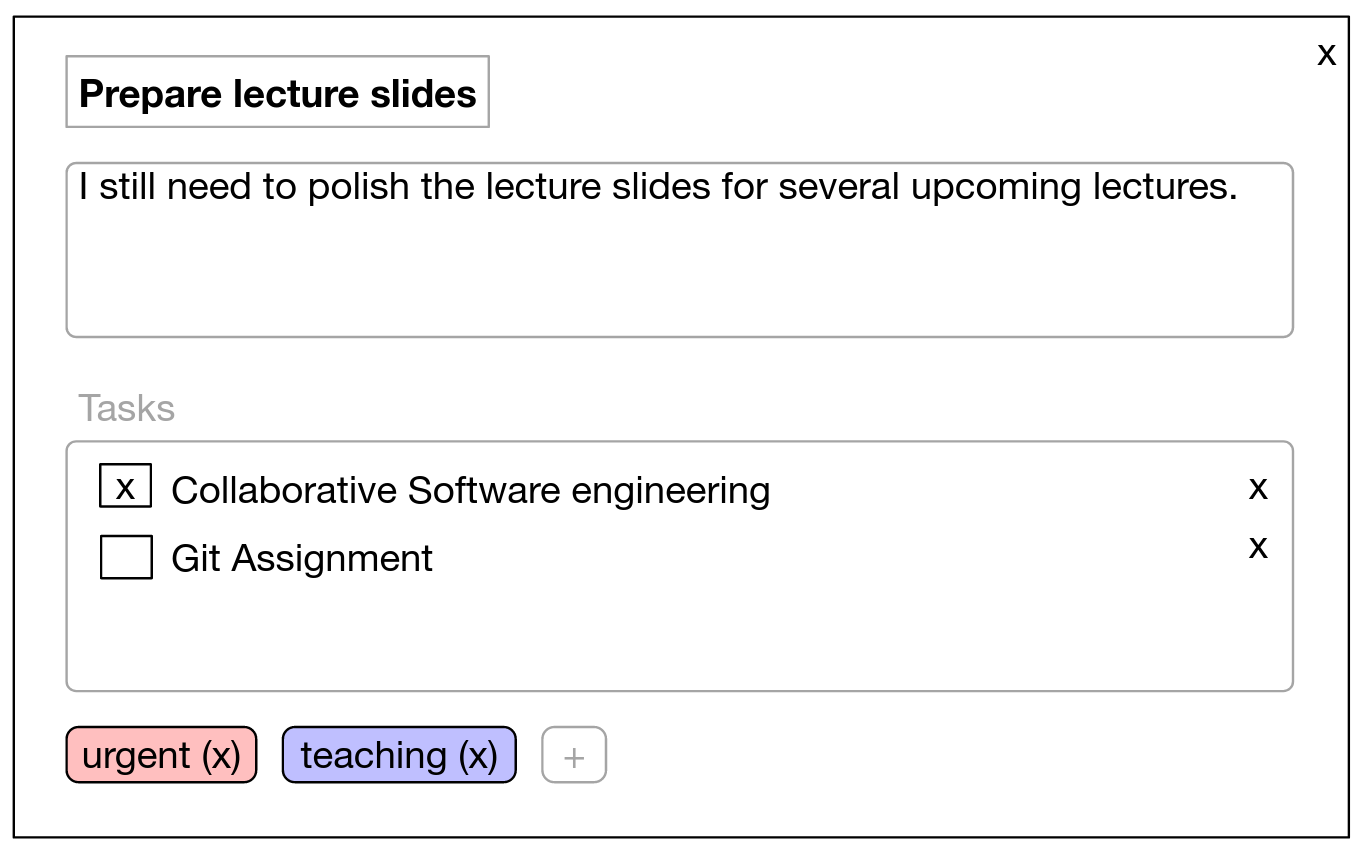
\includegraphics[width=10cm]{mock1}}
		\captionof{figure}{A mock task}
	\end{center}

	\begin{center}
		\shadowbox{
			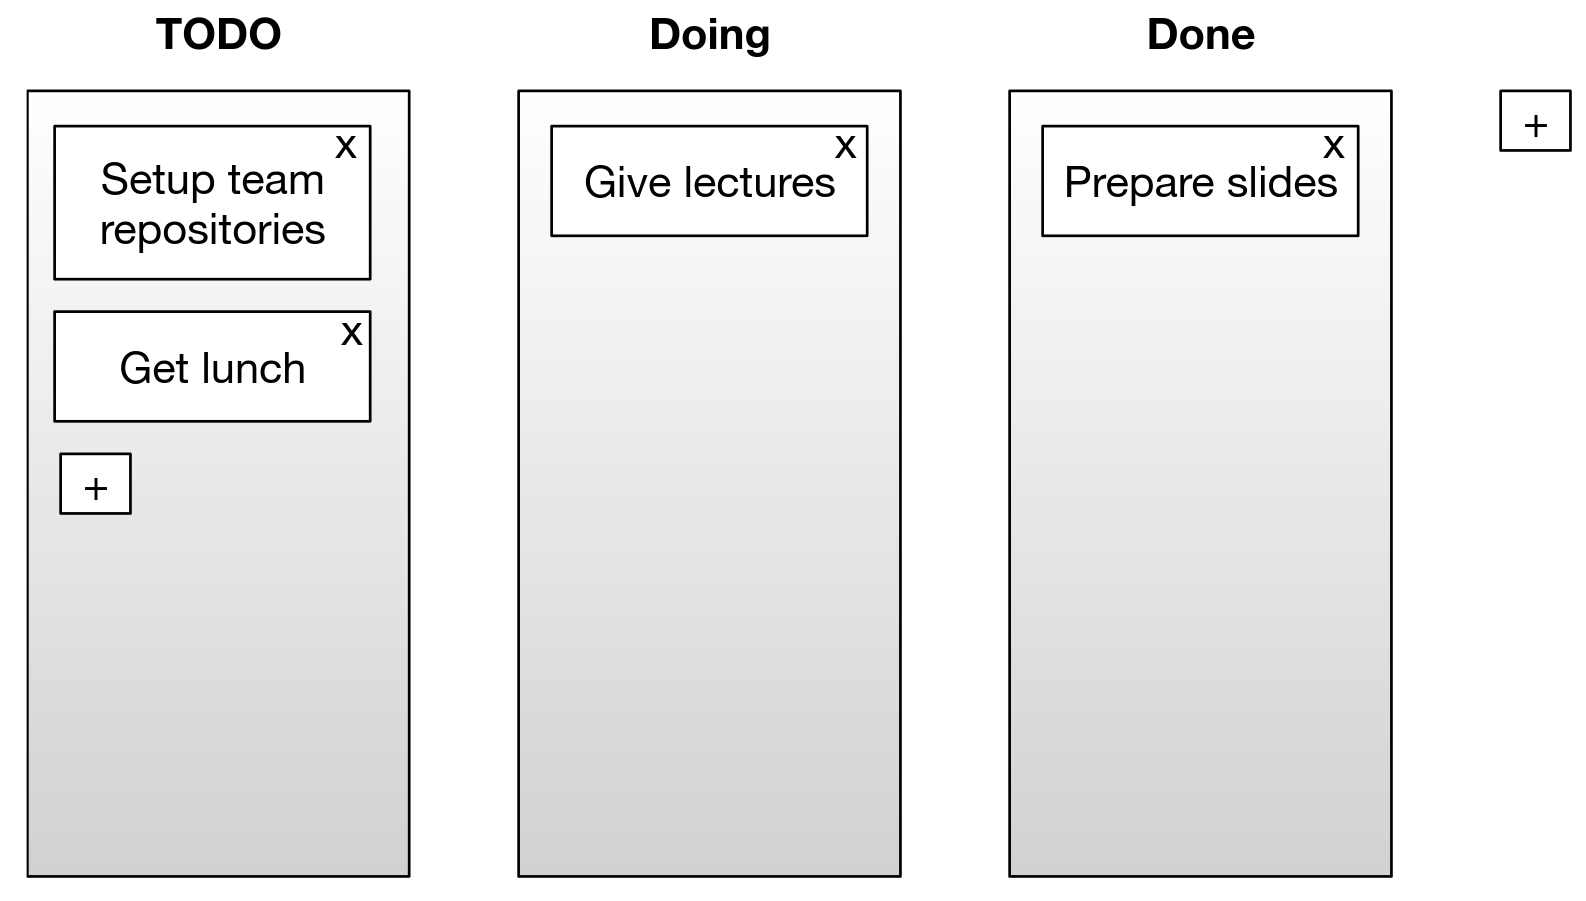
\includegraphics[width=10cm]{mock}}
		\captionof{figure}{A mock of the board}
	\end{center}


	\lfoot{\small \XeLaTeX \hspace{0.1cm} 3.14}

\end{document}
